% Created 2014-01-15 Wed 11:38
\documentclass[11pt]{article}
\usepackage[utf8]{inputenc}
\usepackage[T1]{fontenc}
\usepackage{fixltx2e}
\usepackage{graphicx}
\usepackage{longtable}
\usepackage{float}
\usepackage{wrapfig}
\usepackage[normalem]{ulem}
\usepackage{textcomp}
\usepackage{marvosym}
\usepackage{wasysym}
\usepackage{latexsym}
\usepackage{amssymb}
\usepackage{amstext}
\usepackage{hyperref}
\tolerance=1000
\usepackage{tikz}
\usepackage{tikz}
\usepackage{tikz-cd}
\usetikzlibrary{matrix,arrows,positioning,scopes,chains}
\tikzset{node distance=2cm, auto}
\author{Brian Beckman}
\date{\today}
\title{Fluent, Composable Error Handling}
\hypersetup{
  pdfkeywords={},
  pdfsubject={},
  pdfcreator={Emacs 24.3.1 (Org mode 8.0)}}
\begin{document}

\maketitle
\tableofcontents


\section{Introduction}
\label{sec-1}

Consider a program composed of \emph{serially dependent computations},
any of which produces either a value to send down the line, or an
error. If any computation produces an error, no downstream
computations should be attempted; the error should be the result of
the entire sequence.

We show a sequence of programs in Java and Clojure for this
scenario. We strive for fluent style, which minimizes the number of
temporary variables to name and manage. This style directly mimics
the abstract data flow of the solution.

We find that fluent style is only available in Java if errors are
propagated by exception. Because tht code for handling errors is in
an independent \emph{catch} block, the non-error code path can be written
without explicitly handling errors.

With functional programming in general and Clojure in particular, we
can have fluent code without exceptions because we can delegate
error handling to a monad.
\section{Motivating Example Problem}
\label{sec-2}

As a concrete example, suppose we get an authorization token, do a
database lookup, do a web-service call, filter the results of that
call, do another web-servie call, and then combine the results. The
data flow of our program resembles that in figure
\ref{fig:dataflow}.

\begin{figure}
\begin{center}
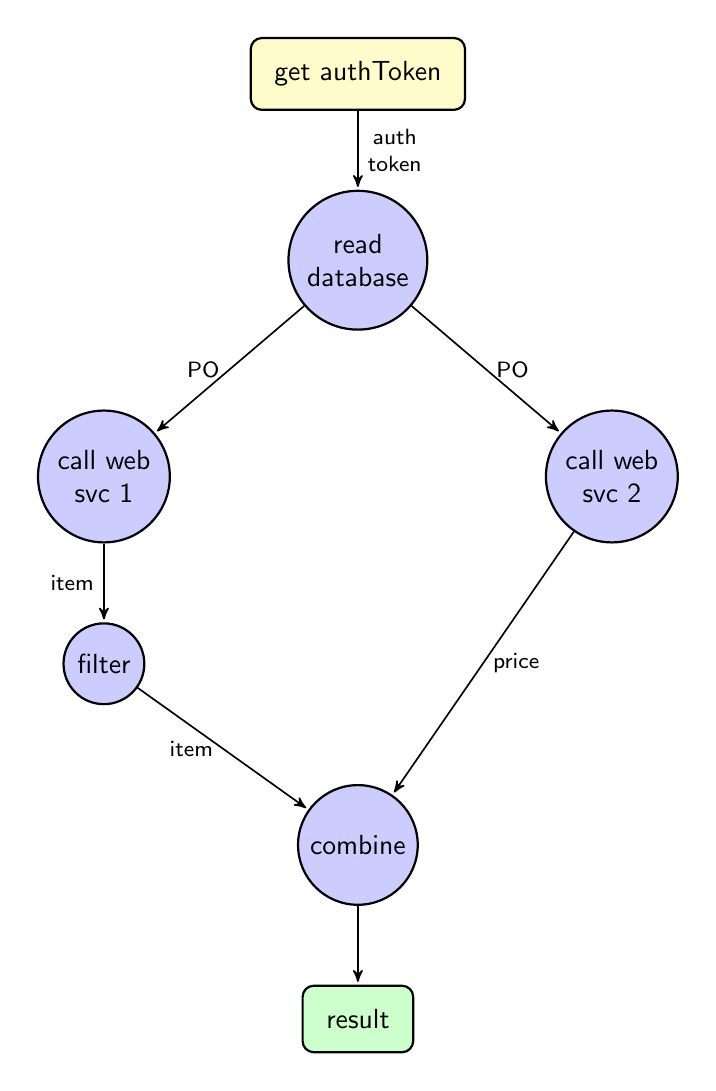
\begin{tikzpicture}[
  font=\sffamily,
  every matrix/.style={ampersand replacement=\&,column sep=1cm,row sep=1cm},
  source/.style={draw,thick,rounded corners,fill=yellow!20,inner sep=.3cm},
  process/.style={draw,thick,circle,fill=blue!20},
  sink/.style={source,fill=green!20},
  rectangle/.style={draw,very thick,shape=rectangle,inner sep=.3cm},
  dots/.style={gray,scale=2},
  invisible/.style={},
  to/.style={->,>=stealth',shorten >=1pt,semithick,font=\sffamily\footnotesize},
  every node/.style={align=center}]

  % Position  nodes using a matrix layout
  \matrix{
      {}
      \& \node[source] (auth) {get authToken};
      \& \\

      {}
      \& \node[process] (database) {read\\database};
      \& \\

      \node[process] (wscall1) {call web\\svc 1};
      \&
      \& \node[process] (wscall2) {call web\\svc 2}; \\

      \node[process] (filter) {filter};
      \&
      \& \node[invisible] (placeholder) {}; \\

      {}
      \& \node[process] (combine) {combine};
      \& \\

      {}
      \& \node[sink] (result) {result};
      \& \\
  };

  % Draw the arrows between the nodes and label them.
  \draw[to] (auth) -- node[midway,right] {auth\\token} (database);
  \draw[to] (database) -- node[midway,left] {PO} (wscall1);
  \draw[to] (database) -- node[midway,right] {PO} (wscall2);
  \draw[to] (wscall1)  -- node[midway,left] {item} (filter);
  \draw[to] (filter)   -- node[midway,left] {item} (combine);
  \draw[to] (wscall2)  -- node[midway,right] {price} (combine);
  \draw[to] (combine)  -- (result);

\end{tikzpicture}
\end{center}
\caption{\label{fig:dataflow}Serially dependent computations}
\end{figure}

\subsection{Fluent Solution in Java, No Error Handling}
\label{sec-2-1}

In the \mbox{C++ -- like} languages, including JavaScript and Java,
we might keep intermediate results in instance variables and model
the flow in object-to-object methods, that is, as
\textbf{transforms}. This style is called \textbf{fluent style}
because the text of the program resembles the flow in the diagram.

Imagine a \emph{main} program like the following, in which each transform
is on its own line, indented from its \emph{source} by one
\mbox{4-space} tab stop. The \textbf{source} of a transform is an
expression that produces an object to feed downstream.
\begin{verbatim}
public static void main(String[] args) {
    Computation databaseResults = new Computation()
        .authorize()
        .readDatabase();
    String result = databaseResults
        .callWebService()
        .filterResults()
        .combineResults(databaseResults
            .callOtherWebService());
    System.out.println(result); }
\end{verbatim}

The correspondence between the diagram of the program and the code
is obvious. The code \emph{looks like} the diagram. Given a change to the
diagrammatic specification, a programmer may propagate the change
straightforwardly to the code due to fluent style.

We save the \emph{Computation} produced by reading the database in its
own local variable, namely \emph{databaseResults}. The dataflow branches
from that result; wd need it twice, once for calling the first web
service and once for calling the second web service. If not for this
branching and recombining of the dataflow, we might have written the
entire program as one, fluent expression with no intermediate
variables.

Also note the non-idiomatic compressed style, minimizing blank lines
and lines with just one closing brace. We adopt this style to save
space in this paper; production versions of such code would have
more white space.

\subsubsection{A Complete Sample Program}
\label{sec-2-1-1}

The following is a complete program that mocks out the database and
web-service results as static JSON objects encoded in strings. This
can be compiled and executed, even online in a sandbox like
\url{http://www.compileonline.com/compile_java_online.php}.

The most important thing to note about this code is that each
method, \emph{e.g.}, \emph{authorize}, \emph{readDatabase}, etc., takes an object
-- implicitly as \emph{this} -- and returns an object. This convention
enables the fluent style by chaining transforms with dot. It so
happens that we return \emph{this} from each method. We could create a
new object in each transform, but it would not simplify the code and
would not give any performance advantage (quite the opposite).
Instead, we propagate values through instance variables, namely
\emph{authToken}, \emph{databaseResults}, etc.
\begin{verbatim}
public class Computation {
    private String authToken;
    private String databaseResults;
    private String webServiceCallResults;
    private String filteredWebServiceCallResults;
    private String otherWebServiceCallResults;

    public Computation () {}
    public Computation authorize() {
        authToken = "John's credentials";
        return this; }
    public Computation readDatabase() {
        databaseResults = "{\"name\":\"John\", \"PO\":\"421357\"}";
        return this; }
    public Computation callWebService() {
        webServiceCallResults =
            "[{\"item\":\"camera\"}, {\"item\":\"shoes\"}]";
        return this; }
    public Computation filterResults() {
        filteredWebServiceCallResults =
            "[{\"item\":\"camera\"}]";
        return this; }
    public Computation callOtherWebService() {
        otherWebServiceCallResults = "{\"price\":\"420.00\"}";
        return this; }
    public String combineResults(Computation other) {
        return "{[" + filteredWebServiceCallResults +
            "," + otherWebServiceCallResults + "]}"; }

    public static void main(String[] args) {
        Computation databaseResults = new Computation()
            .authorize()
            .readDatabase();
        String result = databaseResults
            .callWebService()
            .filterResults()
            .combineResults(databaseResults
                .callOtherWebService());
        System.out.println(result);
}   }
\end{verbatim}
\subsection{Fluent Solution in Java, with Exceptions}
\label{sec-2-2}

The program above has \emph{no} error handling. We \emph{must} have error
handling in real-world programs.

One of the better techniques for error handling in fluent style is
with exceptions. If each sub-computation is responsible for
throwing its own exception, then a single try-catch suffices to get
error details out of the overall sequence, leaving the essential
dataflow unchanged. Our main routine has minimal changes, and
becomes simply
\begin{verbatim}
public static void main(String[] args) {
    try {
        Computation databaseResults = new Computation()
            .authorize()
            .readDatabase();
        String result = databaseResults
            .callWebService()
            .filterResults()
            .combineResults(databaseResults
                .callOtherWebService());
        System.out.println(result); }
    catch (Exception e) {
        System.out.println(e.getMessage());
}   }
\end{verbatim}
Note, in passing, that we ignore resource management (database
connections, sockets, file handles, etc.) in this
paper.\footnote{Idiomatically, resources can be handled in a \emph{finally}
   clause or with Java 7's Automatic Resource Management (ARM). See
   \url{http://bit.ly/15GYkMh}}

Let us give each mocked sub-computation a \mbox{10\%} chance of
erroring, and our entire sample becomes the following:
\begin{verbatim}
import java.util.Random;
public class Computation {
    private String authToken;
    private String databaseResults;
    private String webServiceCallResults;
    private String filteredWebServiceCallResults;
    private String otherWebServiceCallResults;
    private static Random random = new java.util.Random();
    private static Boolean randomlyError() {
        return random.nextDouble() < 0.10; }

    public Computation () {}
    public Computation authorize() throws Exception {
        if (randomlyError()) { throw new Exception("auth errored"); }
        authToken = "John's credentials";
        return this; }
    public Computation readDatabase() throws Exception {
        if (randomlyError()) { throw new Exception("database errored"); }
        databaseResults = "{\"name\":\"John\", \"PO\":\"421357\"}";
        return this; }
    public Computation callWebService() throws Exception {
        if (randomlyError()) { throw new Exception("ws1 errored"); }
        webServiceCallResults =
            "[{\"item\":\"camera\"}, {\"item\":\"shoes\"}]";
        return this; }
    public Computation filterResults() throws Exception {
        if (randomlyError()) { throw new Exception("filter errored"); }
        filteredWebServiceCallResults =
            "[{\"item\":\"camera\"}]";
        return this; }
    public Computation callOtherWebService() throws Exception {
        if (randomlyError()) { throw new Exception("ws2 errored"); }
        otherWebServiceCallResults = "{\"price\":\"420.00\"}";
        return this; }
    public String combineResults(Computation other) throws Exception {
        if (randomlyError()) { throw new Exception("combine errored"); }
        return "{[" + filteredWebServiceCallResults +
            "," + otherWebServiceCallResults + "]}"; }

    public static void main(String[] args) {
        try {
            Computation databaseResults = new Computation()
                .authorize()
                .readDatabase();
            String result = databaseResults
                .callWebService()
                .filterResults()
                .combineResults(databaseResults
                    .callOtherWebService());
            System.out.println(result); }
        catch (Exception e) {
            System.out.println(e.getMessage());
}   }   }
\end{verbatim}
\subsection{Fluency Lost Without Exceptions}
\label{sec-2-3}

Error handling with exceptions is
debatable,\footnote{\url{http://www.joelonsoftware.com/items/2003/10/13.html}}
especially in Java, where runtime exceptions need not be
declared,\footnote{\url{http://bit.ly/1e5P6Cg}} but the alternative of checked
exceptions can be considered harmful.\footnote{\url{http://bit.ly/9NyrdD}}

Worse yet, the semantics of composed locks and exceptions are black
magic. The fundamental reason is that an exception thrown from
inside a lock leaves the program in an indeterminate state for
other threads, with the lock summarily abandoned. There are expert
techniques for mitigating this,\footnote{\url{http://bit.ly/qOO1r}} but a
defensible way out is just to eschew exceptions.

But, rather than join the debate, just imagine that we have decided
against exceptions for whatever reason and try to write reasonable
code.

Add a private \emph{String} field \emph{errorResult}, and let every method
set the error result if and only if it errors. We must change
\emph{combineResults}; it can no longer return just a \emph{String}, but
rather a \emph{Computation}, because it may, itself, produce an error.
Furthermore, we lose the fluent style because every call must be
individually checked.

A particularly nasty way to check every call is as follows:
\begin{verbatim}
public static String computation () {
    Computation c1 = new Computation();
    Computation c2 = c1.authorize();
    if (c2.errorResult.isEmpty()) {
        Computation c3 = c2.readDatabase();
        if (c3.errorResult.isEmpty()) {
            Computation c4 = c3.callWebService();
            if (c4.errorResult.isEmpty()) {
                Computation c5 = c4.filterResults();
                if (c5.errorResult.isEmpty()) {
                    Computation c6 = c3.callOtherWebService();
                    if (c6.errorResult.isEmpty()) {
                        Computation c7 = c5.combineResults(c6);
                        if (c7.errorResult.isEmpty()) {
                            return c7.getResult(); }
                        else {return c7.errorResult;} }
                    else {return c6.errorResult;} }
                else {return c5.errorResult;} }
            else {return c4.errorResult;} }
        else {return c3.errorResult;} }
    else {return c2.errorResult;} }
public static void main(String[] args) {
    System.out.println(computation()); }
\end{verbatim}

This is so intolerable as to barely deserve criticism, despite the
fact that its working set is optimized for the positive
path!\footnote{The error branches are all at addresses far from the
   common-case, non-error branches, which are clustered together for
   maximum locality.} We've lost any correspondence between the
program text and the program specification, \emph{i.e.}, the diagram in
figure \ref{fig:dataflow}. All options for nesting and placement of
curly braces are ludicrous. Changing the computation graph would
entail a sickening amount of work. Code like this is best left to
automatic code generators, if we tolerate it at all.

The prevailing style, nowadays, is to reverse error branches and to
return as early as possible from the main routine. I have reviewed
many instances of this style in shipped code from pre-eminent
shops. Multiple returns were condemned in the dogma of structured
programming. They are also lethal in code that manages
resources,\footnote{\url{http://bit.ly/sAvDmY}}. Despite these drawbacks,
justification for multiple returns is three-fold:
\begin{itemize}
\item it results in linear code that can be read from top to bottom
\item edits to the computation graph entail just adding or subtracting
a localized block of a few lines of code and adjusting a few
temporary variables
\item modern compilers can reverse the branches \emph{again} in the
generated code automatically after
profiling\footnote{\url{http://bit.ly/QkXSM}}
\end{itemize}

This alternative\footnote{favored in the previously cited
   Joel-on-Software blog} is the following:
\begin{verbatim}
public static String computation() {
    Computation c1 = new Computation();
    Computation c2 = c1.authorize();
    if (! c2.errorResult.isEmpty()) {return c2.errorResult;}
    Computation c3 = c2.readDatabase();
    if (! c3.errorResult.isEmpty()) {return c3.errorResult;}
    Computation c4 = c3.callWebService();
    if (! c4.errorResult.isEmpty()) {return c4.errorResult;}
    Computation c5 = c4.filterResults();
    if (! c5.errorResult.isEmpty()) {return c5.errorResult;}
    Computation c6 = c3.callOtherWebService();
    if (! c6.errorResult.isEmpty()) {return c6.errorResult;}
    Computation c7 = c5.combineResults(c6);
    if (! c7.errorResult.isEmpty()) {return c7.errorResult;}
    return c7.getResult(); }
public static void main(String[] args) {
    System.out.println(computation()); }
\end{verbatim}

This, at least, gets rid of the ludicrous nesting, but exposes another
deep weakness: a proliferation of temporary variables to hold the
intermediate \emph{Computations}. Why bother with this when we have no hope
of fluent style? Instead, consider
\begin{verbatim}
public static String computation() {
    Computation c1 = new Computation();
    c1.authorize();
    if (! c1.errorResult.isEmpty()) {return c1.errorResult;}
    c1.readDatabase();
    if (! c1.errorResult.isEmpty()) {return c1.errorResult;}
    c1.callWebService();
    if (! c1.errorResult.isEmpty()) {return c1.errorResult;}
    c1.filterResults();
    if (! c1.errorResult.isEmpty()) {return c1.errorResult;}
    c1.callOtherWebService();
    if (! c1.errorResult.isEmpty()) {return c1.errorResult;}
    c1.combineResults(c1);
    if (! c1.errorResult.isEmpty()) {return c1.errorResult;}
    return c1.getResult(); }
public static void main(String[] args) {
    System.out.println(computation()); }
\end{verbatim}
Edits to the graph now entail even easier edits to the source.

The whole program at this point is the following:

\begin{verbatim}
import java.util.Random;
public class Computation {
    private String errorResult;
    private String result;
    private String authToken;
    private String databaseResults;
    private String webServiceCallResults;
    private String filteredWebServiceCallResults;
    private String otherWebServiceCallResults;
    private static Random random = new java.util.Random();
    private static Boolean randomlyError() {
        return random.nextDouble() < 0.10; }

    public Computation () {errorResult=""; result="no result";}
    public Computation authorize() {
        if (randomlyError()) { errorResult = "auth errored"; }
        authToken = "John's credentials";
        return this; }
    public Computation readDatabase() {
        if (randomlyError()) { errorResult = "database errored"; }
        databaseResults = "{\"name\":\"John\", \"PO\":\"421357\"}";
        return this; }
    public Computation callWebService() {
        if (randomlyError()) { errorResult = "ws1 errored"; }
        webServiceCallResults =
            "[{\"item\":\"camera\"}, {\"item\":\"shoes\"}]";
        return this; }
    public Computation filterResults() {
        if (randomlyError()) { errorResult = "filter errored"; }
        filteredWebServiceCallResults =
            "[{\"item\":\"camera\"}]";
        return this; }
    public Computation callOtherWebService() {
        if (randomlyError()) { errorResult = "ws2 errored"; }
        otherWebServiceCallResults = "{\"price\":\"420.00\"}";
        return this; }
    public Computation combineResults(Computation other) {
        if (randomlyError()) { errorResult = "combine errored"; }
        result = "{[" + filteredWebServiceCallResults +
            "," + otherWebServiceCallResults + "]}";
        return this;}
    public String getResult() {return result;}
    public static String computation() {
        Computation c1 = new Computation();
        c1.authorize();
        if (! c1.errorResult.isEmpty()) {return c1.errorResult;}
        c1.readDatabase();
        if (! c1.errorResult.isEmpty()) {return c1.errorResult;}
        c1.callWebService();
        if (! c1.errorResult.isEmpty()) {return c1.errorResult;}
        c1.filterResults();
        if (! c1.errorResult.isEmpty()) {return c1.errorResult;}
        c1.callOtherWebService();
        if (! c1.errorResult.isEmpty()) {return c1.errorResult;}
        c1.combineResults(c1);
        if (! c1.errorResult.isEmpty()) {return c1.errorResult;}
        return c1.getResult(); }
    public static void main(String[] args) {
        System.out.println(computation());
}   }
\end{verbatim}
\section{Let's Do Better}
\label{sec-3}

Looking back, the main benefits of fluent style are
\begin{itemize}
\item direct correspondence between the program specification and the
program text -- the text \emph{looks like} the diagram
\item edits to the specification and edits to the code are
straightforward and parallel
\item minimal number of temporary variables
\end{itemize}

But we only have fluent style if we use exceptions. Without
exceptions, we're essentially writing assembly language: storing and
combining intermediate results in temporary variables and checking
for errors after every step.

It's possible to do much better, with
and without exceptions, by going \emph{functional}.

In Java, the fundamental modeling tool is the \emph{mutable}, \emph{stateful
object}. Stateful-object programming has many disadvantages:
\begin{itemize}
\item dataflow is awkward to model
\item concurrency requires locks, which are complex; and \emph{global
reasoning}, which is very complex, to avoid deadlock, livelock,
cycles, starvation, priority inversion, etc.
\item concurrency with exceptions is very difficult
\item composing stateful objects, even without concurrency, is
difficult: the operational semantics of even a sequential program
requires \emph{temporal reasoning}, well outside the capabilities of
compilers and programming tools
\end{itemize}

To begin a trek away from stateful-object programming, start with a
question. Why did we use a new instance variable in the object,
\emph{e.g.}, \emph{authToken}, \emph{databaseResults}, \emph{webServiceCallResults},
etc., for each intermediate state? Why not reuse a single variable
for all non-error results? After all, we used a single variable for
the error result?

The reason is that we wanted the individual methods that update
non-error state to be as independent as possible. Though our mocks
don't do so, in a real program, each intermediate computation would
use the result of its predecessors: \emph{readDatabase} would use the
\emph{authToken}, the web-service calls would use \emph{databaseResults} and
so on. With a separate, named variable for each intermediate result,
the correctness of individual sub-computations would be easier to
verify by inspection. With a single, re-used \emph{String} variable,
temporal flow would be even more obscured and the program would be
even more difficult to understand and maintain. It is definitely
worth a few more named variables to make the program easier for the
next programmer tasked with reading the code. Because the only tool
in Java is mutable state, it is hard to do better than a sequence of
instance variables mirroring the sequence of sub-computations.

The essence of the problem is in modeling a \emph{flow} of data through
\emph{transforms} as a flow of data through mutable variables. If,
instead, we invert the paradigm to put the \emph{transforms} under focus,
we sidestep this problem. Doing so requires a language with
first-class transforms, that is, \emph{functions}. Mutable state
variables become immutable function parameters. Thread-safety
becomes automatic and locks do not arise.

\mbox{C\#} has first-class functions, a.k.a. \emph{lambda expressions},
as does \mbox{C++ 11} and as will \mbox{Java 8}. In the mean time,
we can use \emph{Clojure}, a Java-compatible functional language.

As to error handling, fluency is immediate with exceptions, as
before. We achieve fluency for errors-as-return-values with a
\emph{monad}. Despite the name, monads are not exotic or complicated.
They furnish a straight generalization of function composition. Our
monad flows values through the pipeline, applying user-supplied
functions only when an error has not been produced. The
user-supplied functions do not need to check. This monad abstracts
the boilerplate code for checking errors.

Other monads abstract other boilerplate into the monad machinery,
leaving user-supplied code free of clutter. Monads are inherently
stateless, so are not a good fit in stateful-object programming
languages. They are fundamental for concurrent and distributed
programming, and their benefits are evident in functional
programming languages.

\subsection{Fluent Functional Solution With Exceptions}
\label{sec-3-1}

We may write the program with only one intermediate variable, as
before. This variable holds results of the database read, which we
must use for each of the two web-service calls. There are many
techniques for eliminating this variable, such as \emph{memoization},
\emph{common sub-expression elimination}, \emph{lambda lifting}, \emph{the state
monad}, or \emph{parallel composition}. That is for another time and
place. For now, write the flow directly as a sequential composition
of function calls \emph{via} Clojure's \verb|->|, using its \verb|let|
syntax for the one intermediate variable, as follows:

\begin{figure}[H]
\label{functional-main-1}
\begin{verbatim}
(try
  (let [db-results ; be the result of the composition
        (-> (computation)
            authorize
            read-database
            )]
    (-> db-results
        call-web-service
        filter-ws
        (combine (-> db-results
                     call-other-web-service))))
  (catch Exception e (.getMessage e)))
\end{verbatim}
\end{figure}

This looks very much like the fluent Java solution. In Java, we have
fluent streams of items connected by dots. In Clojure, we have the
same fluent streams of items headed by arrows. The fundamental
difference is that Clojure has no instance variables, therefore it
is automatically re-entrant, unlike our Java solution. The semantics
of the Clojure program is evident in the text -- it's a flow of data
through serially dependent computations. There is no temporal
component to the semantics. Contrast with the Java solution, where
we must understand the temporal sequence of operations to
understand the program.

The rest of the Clojure program is as follows. First, declare a
namespace for our symbols to inhabit:

\begin{figure}[H]
\label{functional-helpers-1}
\begin{verbatim}
(ns temp-1.core)
\end{verbatim}
\end{figure}

Define a private symbol, \emph{computation}, to be a function of no
arguments (denoted by the empty square braces) that produces an
empty hash-map (denoted by the empty curly braces).

\begin{figure}[H]
\label{functional-helpers-2}
\begin{verbatim}
(defn- computation [] {})
\end{verbatim}
\end{figure}

Define a private symbol \emph{randomly-error} to be a function of no
arguments that produces \emph{true} if a random double-precision number
is less than $0.10$.

\begin{figure}[H]
\label{functional-helpers-3}
\begin{verbatim}
(defn- randomly-error [] (< (rand) 0.10))
\end{verbatim}
\end{figure}

Define several private symbols to be mocks of functions that produce
application-specific data, or, with $10\%$ probability, throw an
exception. These all use three-term \emph{if}-branch forms, equivalent to Java's
$\langle{}e_1\rangle{}\texttt{?}\langle{}e_2\rangle{}\texttt{:}\langle{}e_3\rangle{}$
operator, taking an expression of Boolean type and two arbitrary
expressions, only one of which is evaluated.

\begin{figure}[H]
\label{functional-helpers-4}
\begin{verbatim}
(defn- authorize [computation]
  (if (randomly-error) (throw (Exception. "auth errored"))
                       {:auth-token "John's credentials"}))
(defn- read-database [auth-token]
  (if (randomly-error) (throw (Exception. "database errored"))
                       {:name "John", :PO 421357}))
(defn- call-web-service [database-results]
  (if (randomly-error) (throw (Exception. "ws1 errored"))
                       [{:item "camera"}, {:item "shoes"}]))
(defn- filter-ws [web-service-call-results]
  (if (randomly-error) (throw (Exception. "filter errored"))
                       [{:item "camera"}]))
(defn- call-other-web-service [database-results]
  (if (randomly-error) (throw (Exception. "ws2 errored"))
                       [{:price 420.00M}]))
\end{verbatim}
\end{figure}

The last application-specific function, \emph{combine} takes two
arguments and combines them.

\begin{figure}[H]
\label{functional-helpers-5}
\begin{verbatim}
(defn- combine [filtered-web-service-results
                other-web-service-call-results]
  (if (randomly-error)
      (throw (Exception. "combine errored"))
      (concat filtered-web-service-results
              other-web-service-call-results)))
\end{verbatim}
\end{figure}

Several improvements are notable in this attempt:
\begin{itemize}
\item first, as stated, with only one exception, state variables have
become immutable parameters to re-entrant functions, purely local
to each transform
\item the one remaining intermediate variable is itself immutable,
removing any need for temporal reasoning -- we only need to
understand dependencies, and they are explicit in the code
\item the code is shorter, less repetitive, less noisy
\item the values of each mock can be modeled directly as hash-maps,
arrays, integers, and decimal numbers like $420.00M$, as opposed
to JSON objects encoded in strings
\begin{itemize}
\item such direct modeling removes the implied need, unstated in our
Java solution, for JSON-processing code
\item such direct modeling also means that we do not need direct Java
interop; our \emph{computation} ``constructor'' just returns an empty
hash-map
\item if we did need need an exising Java class, we would only need to
      \emph{import} the class and change our constructor call from
      \verb|(computation)| to \verb|(Computation.)|, shorthand for \\
      \verb|(new Computation)|
\end{itemize}
\end{itemize}

We continue to use Java's native \emph{Exception} class.
\subsection{Fluent Error Handling Without Exceptions}
\label{sec-3-2}

The improvements above alone justify the Clojure solution over the
Java solution. But the case is really obvious when we get to error
handling without exceptions. In Clojure, we use a variation of
\textbf{the Maybe monad}.\footnote{\url{http://bit.ly/WV02FF}}

Here is the main code:
\begin{figure}[H]
\label{monadic-main}
\begin{verbatim}
(let [db-results
      (=>> (computation)
           authorize
           read-database)]
  (=>> db-results
       call-web-service
       filter-ws
       (combine (=>> db-results
                     call-other-web-service))))
\end{verbatim}
\end{figure}

It looks \emph{just like} the non-monadic code, only with a different
arrow. The prerequisite helpers are as follows:

\begin{figure}[H]
\label{monadic-helpers-1}
\begin{verbatim}
(defn- computation [] (with-em-result {}))
(defn- authorize [computation]
  (with-em-result
    (if (randomly-error) {:error "auth errored"}
                         {:auth-token "John's credentials"})))
(defn- read-database [auth-token]
  (with-em-result
    (if (randomly-error) {:error "database errored"}
                         {:name "John", :PO 421357})))
(defn- call-web-service [database-results]
  (with-em-result
    (if (randomly-error) {:error "ws1 errored"}
                         [{:item "camera"}, {:item "shoes"}])))
(defn- filter-ws [web-service-call-results]
  (with-em-result
    (if (randomly-error) {:error "filter errored"}
                         [{:item "camera"}])))
(defn- call-other-web-service [database-results]
  (with-em-result
    (if (randomly-error) {:error "ws2 errored"}
                         [{:price 420.00M}])))
\end{verbatim}
\end{figure}

All but \emph{combine} are straightforward modifications of the
non-monadic code, simply wrapping their results in a
\emph{with-em-result}. In fact, this wrapping is one of only two things
we must learn about monads: \textbf{it puts values in boxes}.

\subsubsection{Monads Are Values In Boxes}
\label{sec-3-2-1}

An instance of a monad is just a value in a box. Every monad has an
operator, \emph{m-result}, which takes a value and puts it in a
box. All monads work this way: take a value and put it in a box.
The box can be arbitrarily complicated inside, and each type of
monad has its own type of box. But all monads have the \emph{m-result}
operator in common.

The \emph{with-em-result} macro used above is just shorthand \emph{m-result} for
our error-propagating monad. Here is its definition:
\begin{figure}[H]
\label{with-em-result-macro}
\begin{verbatim}
(defmacro with-em-result [expr]
  `(with-monad if-not-error-m (m-result ~expr)))
\end{verbatim}
\end{figure}

Monads have one more essential operator, \emph{m-bind}. This takes two
arguments: a value-in-a-box and a
function-that-puts-a-value-in-a-box. This function's signature is
just like the signature of \emph{m-result}: it takes a value and puts it
in a box. Here we see again the fundamental simplifying idea: put
values in boxes.

Our monad is called \emph{if-not-error-m}. Its \emph{m-result} operator
simply returns its input. This monad's box is an invisible box.
That's ok; monadic boxes can be arbitrarily complicated, including
not complicated at all. A real-world implementation might do
logging as a side-effect. Our monad's \emph{m-bind} takes a
value-in-a-box and a user-supplied function, like the \emph{m-binds} of
all monads. With this monad, \emph{m-bind} applies the user-supplied
function only if the value doesn't have an error in it. Otherwise,
it puts the value, including its error, in a box and passes it down
the line. Since every subsequent element of the pipeline must go
through the very same \emph{m-bind}, the very first error produced in
the pipeline is propagated all the way through. All subsequent
user-supplied functions are sidestepped. If there is no error, it
applies the user-supplied function to the value. The user-supplied
function has the responsibility of putting the value in a box,
automated by our \emph{with-em-result} macro.
\begin{verbatim}
(defmonad if-not-error-m
  [m-result (fn [value] value)
   m-bind   (fn [value f]
              (if-not (:error value)
                (f value)
                (m-result value)))
  ])
\end{verbatim}

We can see how our new arrow operator, \verb|=>>|, composes values
through \emph{m-bind}. For instance, the fragment

\begin{verbatim}
(=>> (computation)
      authorize
      read-database)
\end{verbatim}
expands approximately to
\begin{verbatim}
(with-monad if-not-error-m
  (m-bind
    (m-bind (computation)
            (fn [temp] (authorize temp)))
    (fn [temp] (read-database temp))))
\end{verbatim}
Longer chains expand to more deeply nested compositions of \emph{m-bind}
behind the scenes, precisely where it should be. Contrast this to
the Java situation, where we had no tools in the language for
mitigating intolerable nesting and proliferation of temporaries.
Here, we define our arrow directly in our application code.
Clojure, in particular, and homoiconic
languages,\footnote{\url{http://en.wikipedia.org/wiki/Homoiconicity}} in
general, often have embedded rewrite
systems\footnote{\url{http://en.wikipedia.org/wiki/Rewriting}} or macro
languages.\footnote{\url{http://en.wikipedia.org/wiki/Macro_(computer_science)}}
Without going more deeply into Clojure's macro syntax or the
monadic \emph{m-chain} helper it employs, the arrow macro is at least
small:
\begin{verbatim}
(defmacro =>> [in-monad & transforms]
  `(with-monad if-not-error-m
     ((m-chain [~@transforms]) ~in-monad)))
\end{verbatim}

The final monadic helper, \emph{combine}, illustrates \emph{m-bind} directly.
Given a value from the second of the two web-service calls, it
produces a \emph{closure}
\footnote{\url{http://en.wikipedia.org/wiki/Closure_(computer_science)}}
a first-class value of type
\emph{function-that-puts-a-value-in-a-box}. That function
will be composed, \emph{via} \emph{m-bind}, with the filtered value of the first
of the two web-service calls. We use the suffix \emph{-val} to
distinguish values-not-in-boxes from value-in-boxes, which are
produce by \emph{with-em-result}.
\begin{figure}[H]
\label{monadic-helpers-2}
\begin{verbatim}
(defn- combine [other-ws-results-val]
  (fn [filtered-ws-results-val]
    (with-em-result ; produces a value-in-a-box
      (if (randomly-error)
        {:error "combine errored"}
        (concat filtered-ws-results-val
                other-ws-results-val)))))
\end{verbatim}
\end{figure}
\subsubsection{Monad Particulars and Generalities}
\label{sec-3-2-2}

The implementations of \emph{m-result} and \emph{m-bind} are particular to
each monad. Package your application-dependent logic in
user-supplied functions-that-put-values-in-a-box. Compose them \emph{via}
\emph{m-bind}, \emph{m-chain}, or the \verb|=>>| operator.
\subsubsection{Varying from the Standard Maybe Monad}
\label{sec-3-2-3}

Why do we have a variation of the standard \emph{Maybe} monad? Why not
just use \emph{Maybe}? First, \emph{Maybe} produces an unadorned \emph{Nothing} if
anything goes wrong. The consumer of the computation doesn't know
what stage of the pipeline failed nor any details at all about the
error. Such is not tolerable in the real world. In our example of a
database read followed by web-service calls followed by filtering
and combining, if something goes wrong in this sequence of
computations, we need to know exactly where and to log as much
detail as we can get about the failure. But we certainly don't want
any computations downstream of the failure to be attempted. We
want the pass-through semantics of \emph{Maybe} but without the ignorance.
\section{Conclusion}
\label{sec-4}

Controlling complexity is the central problem of software
engineering. Making code closer to specifications is essential, and
that is the central theme of progress in programming languages.

Many business processes are fundamentally data-flows. Modeling
data-flows directly in our programming languages and applications is
a clear advantage.

Fluent style is a direct representation of dataflow dependencies in
the text of a program. Stateful-object programming is an awkward fit
to fluent style. The semantics of stateful-object programs are
temporal and implicit, while the semantics of fluent style are
dependency-based and explicit.

Fluent style can be approached in stateful-object programming by
simulating flow-through-transforms as
flow-through-instance-variables, but the style is brittle. For
instance, changing from errors-as-exceptions to
errors-as-return-codes makes fluent style intractable.

Furthermore, tateful-object programming makes concurrency more
hazardous. Composability of objects and exceptions is difficult to
test, and manual, pattern-based concurrent programming with locks is
a dark art for the elite few. Yet, concurrency is necessary in
everyday web programming.

In addition to enabling fluent style everywhere, functional
programming aleviates the other hazards of stateful-object
programming. It is composable both with exceptions and with
errors-as-return-codes. Because function-parameters are immutable,
functions are naturally re-entrant. Functional programming also
sidesteps the temporal reasoning required for stateful-object
programming, making code easier to test and debug.
% Emacs 24.3.1 (Org mode 8.0)
\end{document}
